
\documentclass[]{article}

\title{Tarea 1 de modelos probabilistas aplicados}
\author{Joaquin Arturo Velarde Moreno}

\date{}
\usepackage{braket}
\usepackage{bbold}
\usepackage{amsmath,amsfonts,amssymb,amsthm}
\usepackage[margin=1.0in]{geometry}
\usepackage{graphicx}
\usepackage{chngcntr}

\usepackage[backend=biber]{biblatex}
\addbibresource{ref.bib}
\begin{document}
	\maketitle
	\begin{center}
		\line(1,0){200}
		\linebreak
		\linebreak
		\linebreak
		\textsc{\Large Análisis de Visitantes internacionales que ingresaron al país en el 2020}
	
	\end{center}

\section{Origen de los datos}
	Los datos que a continuación se analizaran fueron obtenidos de la pagina del INEGI\cite{inegi}, en su apartado de turismo, estos son obtenidos gracias a las encuestas de viajeros internacionales en las fechas de agosto 2018 a junio 2020 y después publicadas en formatos XLSX.
	
	\section{Uso de los datos}
	
	Se hizo un enfoque en el año 2020 aislando esta sección de datos de los demás y siendo generado y editado por Microsoft Excel\cite{excel}, este solo provee información preliminar de los meses Enero, Febrero, Marzo, Abril, Mayo, Junio. 
	\linebreak
	se creo un diagrama de cajas y bigotes con el cual se puede representar de manera visual el conjunto de visitantes por mes y obtener los siguientes datos: minimo, maximo, media, primer cuartil y tercer cuartil, la herramienta para su análisis fue R version 4.0.2\cite{rproject}.

	En la figura \ref{fig:mesh} se puede observar los datos clasificados en turistas de internación, turistas fronterizos, Excursionistas fronterizos y Excursionistas en cruceros.

	\subsection{turistas de internación}
Los turistas de internación los cuales son los que se adentran dentro del territorio del país tienen métodos de ingreso la vía aérea y la vía terrestre, en este se puede concluir que el método preferido es el aéreo.

	\subsection{turistas fronterizos}
Los turistas fronterizos son aquellos que viajan a las ciudades fronterizas de nuestro país por desplazándose de manera peatonal o automovilística mente.

	\subsection{Excursionistas fronterizos}
Los Excursionistas fronterizos son aquellos que principalmente cruzan la frontera para hacer compras y regresar a su país sin quedarse una noche desplazándose de manera peatonal o automovilística mente.

	\subsection{Excursionistas de crucero}
	Los Excursionistas de crucero son pasajeros que visitan un puerto mexicano sin quedarse la noche en México, su manera de proceder consiste en llegar al puerto, conocer, hacer compras y regresar al crucero, es interesante resaltar que debido a la crisis sanitaria del COVID-19 en los Últimos meses el numero de excursionistas de crucero ha sido de 0.
\section{Gráfico}	
	\counterwithin{figure}{section}
	\begin{figure}[h]
    	\centering
    	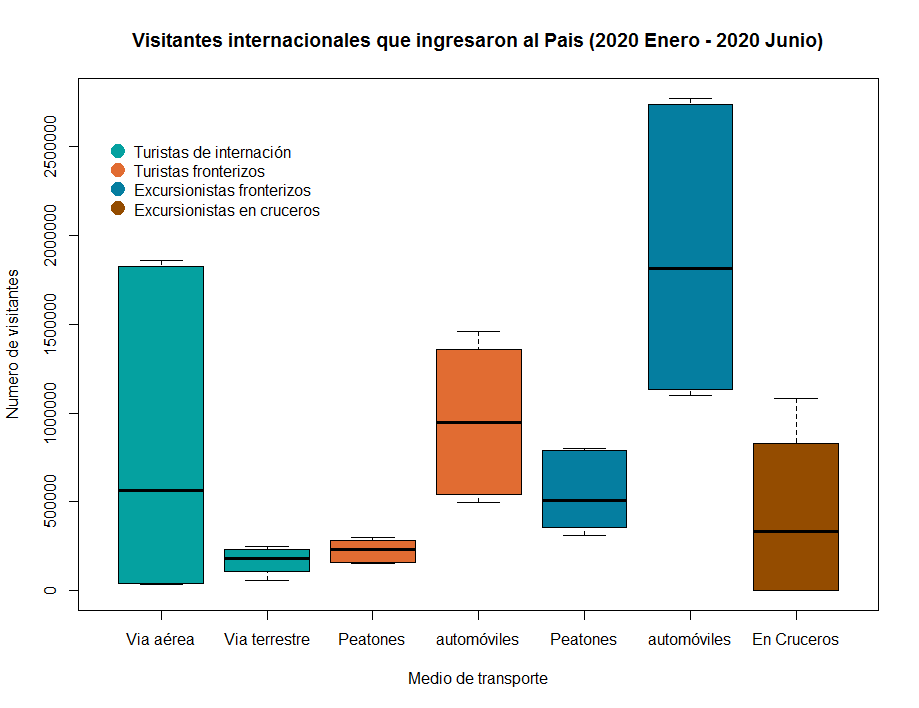
\includegraphics[scale=.5]{Turismo}
    	\caption{Visitantes internacionales por tipo}
    	\label{fig:mesh}
	\end{figure}

\printbibliography[title={Referencias}]
\end{document}
